\documentclass[9pt,twocolumn,twoside,lineno]{new_article}

% Use the lineno option to display guide line numbers if required.

% packages
\usepackage{courier}
\usepackage{multirow}

\title{Genomic architecture controls multivariate adaptation to climate change}

% Use letters for affiliations, numbers to show equal authorship (if applicable) and to indicate the corresponding author
\author[a,b,c,1]{Drew E. Terasaki Hart}
\author[a]{Ian J. Wang}

\affil[a]{Department of Environmental Science, Policy, and Management, University of California, Berkeley, CA 94720, USA}
\affil[b]{The Nature Conservancy, Arlington, VA 22203, USA}
\affil[c]{Commonwealth Scientific and Industrial Research Organisation, Ecosciences Precinct, Dutton Park, QLD 4102, Australia}

% Please give the surname of the lead author for the running footer
\leadauthor{Terasaki Hart} 

% Please include corresponding author, author contribution and author declaration information
\authorcontributions{D.E.T.H. conceived, designed and wrote the simulations and analysis, and wrote the manuscript. I.J.W. helped conceive and design the simulations and analysis, and cowrote the manuscript.}
\authordeclaration{The authors declare no competing interests.}
\correspondingauthor{\textsuperscript{1}To whom correspondence should be addressed. E-mail: drew.hart@berkeley.edu}

% At least three keywords are required at submission. Please provide three to five keywords, separated by the pipe symbol.
\keywords{adaptation $|$ climate change $|$ $|$ landscape genomics $|$ spatial simulation $|$ gene flow $|$ genomic architecture $|$ genetic redundancy} 

\begin{abstract}
As climate change advances,
environmental gradients may decouple,
generating novel multivariate 
environments that stress wild populations.
A commonly invoked mechanism of evolutionary rescue is adaptive gene flow
tracking climate shifts, but gene flow from populations inhabiting similar conditions on one environmental axis could cause maladaptive introgression when populations are adapted to different environmental variables that do not shift together.
Genomic architecture can play an important role in
determining the effectiveness and relative magnitudes of adaptive gene flow and \textit{in situ} adaptation.
This may have direct consequences for how species respond to climate change, but is often overlooked.
Here, we simulate microevolutionary responses to environmental change
under scenarios defined by variation in the polygenicity, linkage, and genotypic redundancy of two independent traits,
one of which in adapted to a gradient that shifts under climate change.
We use the ensemble of simulations to examine how genomic architecture influences evolutionary outcomes under climate change.
We found that climate-tracking (up-gradient) gene flow, though present in all scenarios,
was strongly constrained under scenarios of lower linkage and higher polygenicity and redundancy,
suggesting \textit{in situ} adaptation
as the predominant mechanism of evolutionary rescue under these conditions.
We also found that high polygenicity
caused increased maladaptation and
demographic decline, a concerning result given that many climate-adapted traits may be polygenic.
Finally, in scenarios with high redundancy we observed increased adaptive capacity
and reduced up-gradient gene flow.
This finding adds to the growing recognition of the importance of redundancy,
imputes to redundancy a key role in mediating \textit{in situ} adaptive capacity,
and thus suggests opportunities for better understanding the climatic vulnerability of real populations.
\end{abstract}



\dates{This manuscript was compiled on \today}

\begin{document}

\maketitle
\thispagestyle{firststyle}
\ifthenelse{\boolean{shortarticle}}{\ifthenelse{\boolean{singlecolumn}}{\abscontentformatted}{\abscontent}}{}


\dropcap{C}limate change is one of the foremost threats to biodiversity in the Anthropocene.
The ability of species to persist within their current ranges will likely depend largely upon their abilities to
locally adapt to new climate conditions --- a concept frequently referred to 
as `adaptive capacity’ or `evolutionary potential’ \cite{chevin,harrisson,nicotra,vilas,wade}.
Because beneficial \textit{de novo} mutations take a long time to arise,
this adaptation will instead most likely be facilitated
by the reconfiguration of existing adaptive genetic diversity \cite{bomblies}.
A common conceptual model underlying this scenario is that of
adaptive gene flow tracking a shifting climatic gradient
(i.e., in the vector
direction of climate velocity; \cite{loarie,ackerly}),
which would bring beneficial genes into recipient populations
from `climate-suitable' populations --- i.e., populations whose
current climates approximate future local conditions \cite{bellis}.
This model of adaptive gene flow has both theoretical
\cite{aitken_whitlock,slatkin,tigano}
and empirical 
\cite{feder,bell}
support
but meets resistance under theoretical conditions in which gene flow can be maladaptive
\cite{wang,lenormand,slatkin,haldane,wright,felsenstein}.
In these circumstances, shifting allelic covariance --- 
 the \textit{in situ} recombination of standing genetic variation into new,
adaptive genotypes --- could be a more efficient mechanism of local adaptation to environmental change.

In recent decades, research bridging the fields
of molecular population genetics
and quantitative genetics
\cite{barghi_polygenic,barton,pritchard_human_adaptation,pritchard_sweeps_alone}
has revealed that the genomic architecture of a trait
is a core determinant of whether and how that trait
becomes locally adapted \cite{yeaman_review}.
Among the key aspects of genomic architecture that influence adaptation
\cite{barton,yeaman_whitlock,yeaman_review,lecorre} are:
the number of loci underlying a trait (henceforth, `polygenicity'),
the rate of recombination between these loci (i.e., linkage),
and the number of distinct genotypes that yield identical phenotypes
(henceforth, `genotypic redundancy').
(We note that we use the term `genotypic redundancy',
\textit{sensu} Láruson et al. 2020 \cite{laurson},
rather than the more familiar but more general term `genetic redundancy',
because it provides conceptual and quantitative precision
that correctly describes the design of our simulations.)
Previous research suggests that ecologically-important traits can vary from having
few loci of large effect \cite{martin,rees}
to many loci of small effect \cite{boyle,rockman,savolainen,sella,barghi_polygenic},
and shows that this variation in polygenicity can
determine the rate and nature of local adaptation \cite{yeaman_amnat}. 
Linkage controls the likelihood that adaptive alleles cluster together,
essentially forming alleles of larger effect size that are stronger 
targets of selection and more resistant
to swamping gene flow \cite{yeaman_whitlock},
thereby facilitating local adaptation \cite{tigano}.
Genotypic redundancy can facilitate local adaptation 
by allowing the existence of a stable phenotypic cline
subtended by a genetic dynamic equilibrium
consisting of continuous and concerted shifts in non-neutral allele frequencies
\cite{barghi_redundancy,manceau,yeaman_amnat}.
We refer to this phenomenon as `transient genomic architecture'.

The influence of genomic architecture on the nature and outcomes
of local adaptation to changing environmental gradients
has been studied to a limited extent,
with nearly exclusive focus on univariate models
of the selective environment (but see \cite{schiffers}).
Yet, such models have limitations for studying adaptation to climate change
because, in nature, species can be adapted simultaneously to multiple,
independent environmental gradients \cite{guillaume} that can shift differentially,
and thus decouple, as climate change advances
\cite{crimmins,daly},
leading to the emergence of novel multivariate landscapes
\cite{williams_novel_climates,williams_projected_novel_disappearing,fitzpatrick}.
Thus, it is important to investigate how the genomic architectures
of multiple traits can combine to determine the nature and outcome
of multivariate adaptation under climate change.
Gene flow from `climate-suitable' portions of a species' range
is often assumed to be beneficial for adaptation to climate change.
This may be accurate from the perspective of a single trait
adapted to a shifting climatic gradient, but it may be
an invalid assumption if the gene flow also carries
linked variation for a trait
adapted to a second environmental variable
from which the shifting gradient has decoupled.
If the latter is true,
then gene flow may introduce alleles for the second trait
that are disadvantageous and that could counteract any fitness advantage
gained with respect to the first trait.
Thus, the genomic architectures of both traits
may determine the overall evolutionary outcomes
by controlling the relative likelihoods of adaptation by gene flow
and of \textit{in situ} adaptation by shifting
allelic covariance
\cite{aitken_whitlock,schiffers}.

Spatially-explicit simulation is one of our strongest tools
for improving our understanding of the complex dynamics of gene flow and adaptation
under climate change \cite{capblancq_review}.
In this study, we use individual-based, spatially-explicit simulations,
constructed in \texttt{Geonomics} \cite{terasaki_hart},
to test how genomic architecture influences multivariate adaptation to climate change.
We simulate the adaptation of a single population
continuously distributed on a two-dimensional landscape composed of two different environmental
variables, each one being a gradient that runs parallel to the x-axis and that exerts selection on a separate trait.
In our main models, we then simulate climate change on that landscape by holding one gradient 
constant while gradually shifting the other gradient along the x-axis, such that
the decoupling environment pushes local fitness peaks toward novel regions 
of two-dimensional trait space (Fig. \ref{fig:fig_1}).
We run 100 pairs of climate change simulations
and null (i.e., stable climate) simulations for each of eighteen scenarios
resulting from the full factorial crossing of three key components
of genomic architecture: genotypic redundancy, polygenicity, and linkage
(Table \ref{tab:tab_1}).

\begin{table}
\begin{tabular}{b{0.35\linewidth}b{0.05\linewidth}b{0.45\linewidth}}
\hline
\textbf{component} & \textbf{level} & \textbf{parameter value} \\
\hline
\multirow{2}{10em}{genotypic redundancy} \\
& low: & $\texttt{redund}=1$ \\
& high: & $\texttt{redund}=2$ \\
\hline
\multirow{2}{10em}{polygenicity} \\
& low: & $\texttt{n\_loci}=4\times \texttt{redund}$ \\ 
& mod: & $\texttt{n\_loci}=20\times \texttt{redund}$ \\
& high: & $\texttt{n\_loci}=100\times \texttt{redund}$ \\
\hline
\multirow{2}{10em}{linkage} \\
& low: & $\texttt{recomb}=0.5$ \\
& mod: & $\texttt{recomb}=0.05$ \\
& high: & $\texttt{recomb}=0.005$ \\
\hline
\end{tabular}
\medskip
\caption{\label{tab:tab_1}Parameter values used for each of the three focal components of genomic architecture. The full factorial combinations of these parameter values constitute the set of 18 simulation scenarios for which we present results.}
\end{table}

\begin{figure}%[tbhp]
\centering
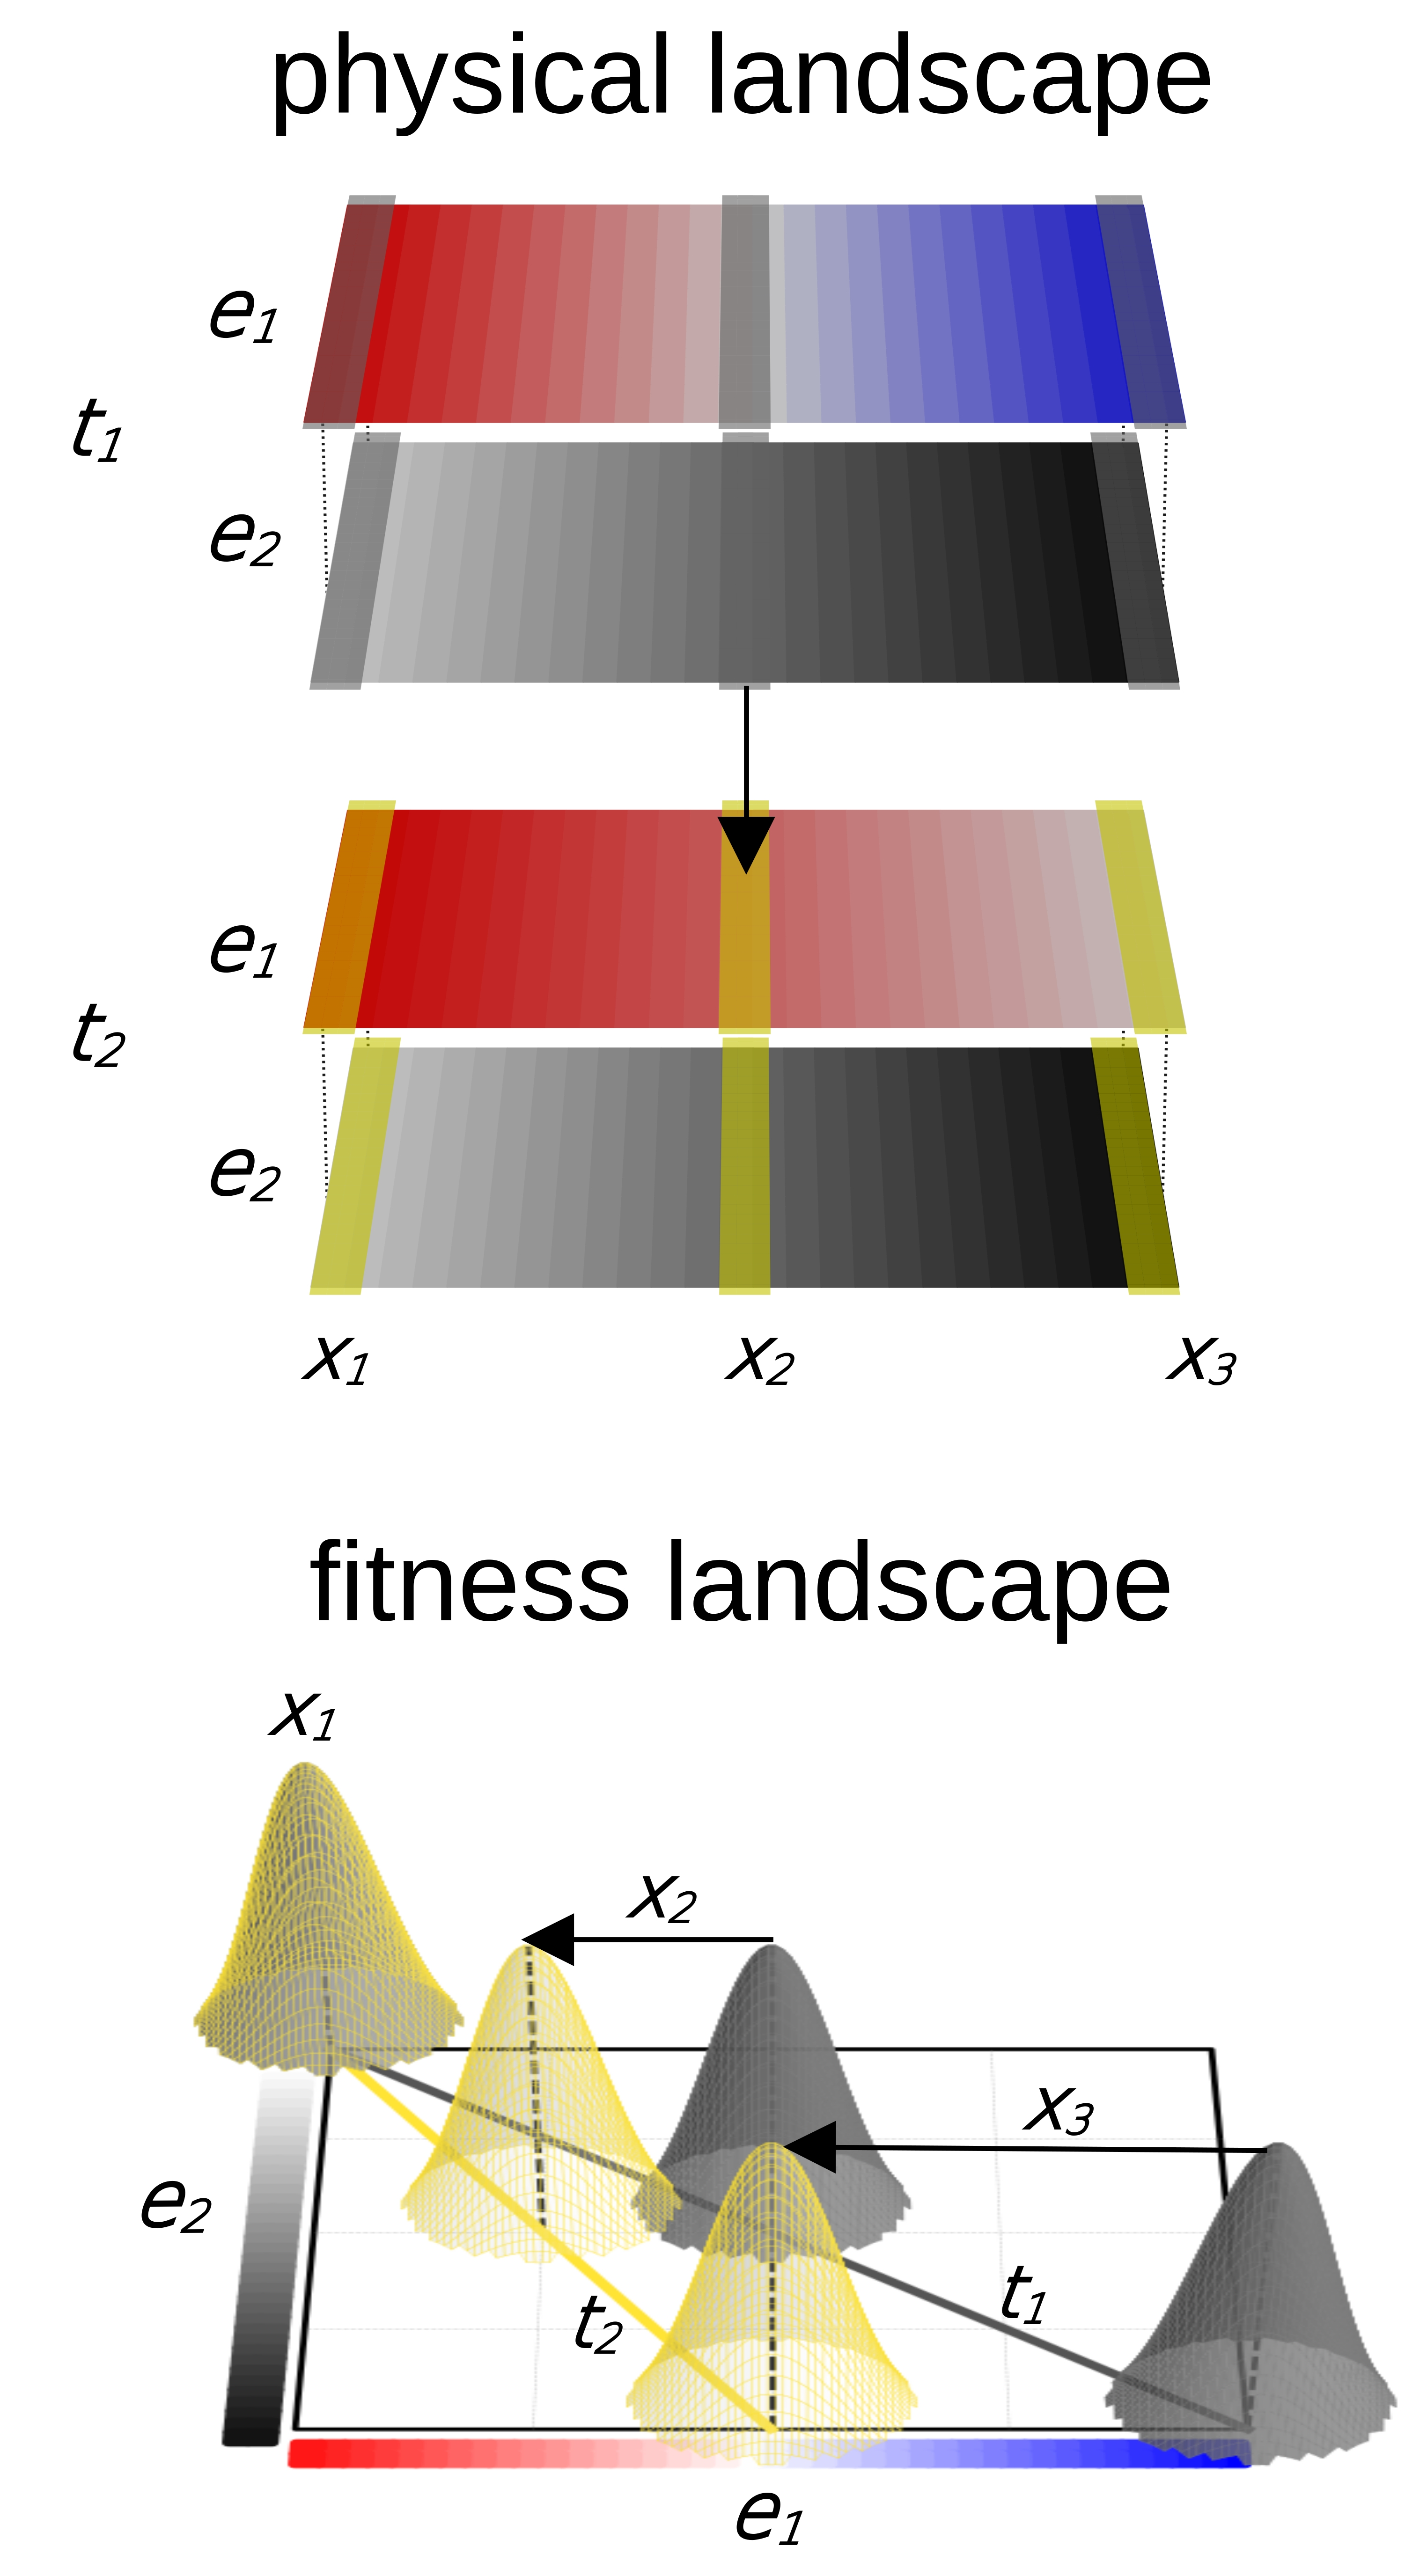
\includegraphics[width=.8\linewidth]{pub/figs_and_stats/FIG_1_conceptual.jpg}
    \caption{Conceptual model of adaptation to climate change. The top panel depicts the two-layered physical landscape used in our simulations, showing the shifting environmental gradient ($e_{1}$) in a blue-red color ramp and the stable gradient ($e_{2}$) in a white-black color ramp. The landscape is shown both before climate change ($t_{1}$) and after ($t_{2}$). The bottom panel depicts a fitness landscape for two traits adapted to the shifting ($e_{1}$) and stable gradients ($e_{2}$). Three example positions on the physical landscape ($x_{1}$, $x_{2}$, $x_{3}$) are shown as boxes delinated y-axis cross-sections, both before climate change (gray) and after (yellow), and their corresponding fitness peaks are shown as color-matched kernels on the fitness landscape. The gray and yellow lines on the fitness landscape indicate the fitness optima defined by the environments that exist before ($t_{1}$) and after climate change ($t_{2}$). Shifts in local fitness peaks are shown as labeled arrows ($x_{2}$, $x_{3}$); the environment at the far left of the physical landscape does not change, so $x_{1}$'s fitness peaks are overlapping and have no shift.}
\label{fig:fig_1}
\end{figure}


We analyze cross-scenario variation in the resulting spatiotemporal
patterns of gene flow, population size and density, and phenotypic
distributions --- all of which are emergent properties of our simulation
parameterizations (Code Sample S1) --- 
to test a series of hypotheses about the influence of genomic architecture 
on multivariate adaptation under climate change. First, we hypothesize that up-gradient 
gene flow will be higher under climate change than under a stable climate across all
scenarios but that gene flow contributes least to climate change adaptation when
linkage is low and polygenicity is high.
This is because we expect gene flow to always have
at least some adaptive value, but we also expect low-linkage, high-polygenicity architectures 
(i.e., 'dispersed' architectures \cite{yeaman_review}) to exhibit quick \textit{in situ}
adaptation via shifting allelic covariance among many small-effect alleles, akin to adaptation 
under transient genomic architectures, facilitating phenotypic shifts in the absence of up-gradient gene flow.
Second, we hypothesize that stronger linkage 
and higher polygenicity will reduce a population's adaptive capacity under climate change,
manifesting as greater reductions in population size and mean fitness
and more persistent maladaptation, because both conditions impose longer expected
wait times for the emergence of recombinant haplotypes that push phenotypes
further from their pre-change fitness peaks. Finally, we hypothesize that higher genotypic redundancy
will facilitate adaptation to shifting gradients, much as it does on stable gradients 
\cite{barghi_redundancy,manceau,yeaman_amnat}, resulting in smaller reductions 
in population size and mean fitness.


\section*{Methods}

\subsection*{Simulations}

We performed simulations using \texttt{Geonomics} \cite{terasaki_hart},
a Python \cite{rossum} package for forward-time, agent-based, continuous-space landscape genomic simulations.
All of our simulated scenarios feature
a species with two traits, each of which experiences 
selection on the basis of a different environmental variable.
Both environmental variables are modeled as linear gradients running along the x-axis
that initially span environmental values from 1 to 0, left to right across the landscape.
The genome is modeled as an array of length L,
which in our 2-trait simulations equals 2 times the number of genes per trait.
Instead of randomly assigning loci to either of the two traits
we alternate locus trait assignment along the genome,
to avoid creating islands of within-trait linkage
that would vary across iterations and introduce noise in our results.
The fitness of individuals is a function of the difference between their local
environmental values and their phenotypes, which are determined by the
additive effects of multiple loci (i.e., without pleiotropy or epistasis), a reasonable approximation of many traits in real populations \cite{sella}.
(While two linked genes underlying dinstinct traits may behave similarly to pleiotropy,
it is a distinct phenomenon subject that may emerge within our models but that is subject to erosion by recombination;
we do not model pleiotropy \textit{sensu stricto}.)
Local environmental values are derived from the landscape cells within which individuals' locations fall.
Individuals' locations update during each time step's movement phase,
when each individual moves along a vector composed of a randomly drawn direction
(from a uniform circular distribution) and a randomly drawn distance
(from a Wald(0.25, 0.5) distribution, such that most movements are less than one landscape cell in length).

Simulations start with a neutral burn-in period that does not include differential fitness.
The burn-in is concluded when statistical tests
of temporal and spatial population stability are passed,
at which point individuals are randomly assigned genomes
based on 0.5|0.5 allele frequencies at all loci.
Simulations then run for 2500 time steps with differential fitness,
generating a pattern of local adaptation to the initial environment.
After that, one environmental layer undergoes a change 
event in which the gradient’s values change stepwise over a period of 250 time steps,
resulting in a final gradient that spans values from 1 to 0.5, left to right.
This creates a scenario in 
which the two environmental variables become decoupled, leading 
to the emergence of novel environments (i.e. sites occupying new values in 
two-dimensional environmental space).
The purpose of this is to emulate a common 
phenomenon under climate change: the decoupling of multivariate environmental gradients,
leading to the emergence of novel conditions
\cite{williams_novel_climates,williams_projected_novel_disappearing,fitzpatrick}.
This generates spatially heterogeneous rates of climate change, ranging from no change at the leftmost edge to 0.002 units per timestep at the rightmost edge.
We chose this scenario because one with spatially homogeneous rates of change would generate an artefact of range expansion
whose genomic signal could not reliably be disentangled from that of
climate change adaptation. Hence, the approach we chose here allows us
to isolate the evolutionary dynamics
resulting from the components of genomic architecture
that define our scenarios and hypotheses.
(We note that the pre-climate change population sizes in our simulations,
stochastically varying around 5800-6100 individuals,
yield mean expected allelic persistence times
on the order of 16000-17000 time steps \cite{wright,terasaki_hart},
roughly an order of magnitude larger than our total runtime,
precluding concern for substantial drift-driven diversity loss during simulations.)

We used a custom Python script to establish values for the parameters of interest in our simulations: the number of loci underlying
each trait (parameter \texttt{n\_loci}),
the recombination rate between neighboring loci
(parameter \texttt{recomb}),
and the level of genotypic redundancy (parameter \texttt{redund}).
The values we assign to these parameters are provided in Table \ref{tab:tab_1}, and a visual depiction, across all possible phenotypes, of the difference between low- and high-redundancy scenarios is provided in Fig. S1.
We used that script to run the simulations on the 
savio3 partition of UC Berkeley’s Savio computing cluster (each node has 96 GB RAM and 32, 
2.1-GHz Skylake processors). For each scenario, we ran a total of 100 iterations, featuring a 250 time-step climate change period (henceforth, 
the ‘main’ scenarios), and 100 iterations of a paired null scenario without natural 
selection (henceforth, the ‘null’ scenarios). 
\texttt{Geonomics} is a complex simulation framework that features numerous other 
parameters; we set those at their default values.
Some values of interest that might be explicit parameter settings in
other simulation programs are instead
emergent properties in \texttt{Geonomics}; for example, the population size values we report emerge from the interaction
of several explicit parameters, including the raster of local carrying capacities,
the population intrinsic growth rate, the number of offspring per reproduction event,
and the death rates resulting from the parameters controlling density-dependent mortality
and natural selection.
The complete set of \texttt{Geonomics} parameters and the values 
we assigned to them across all models are provided in Code Sample S1.
Values parameterize a scenario that can be considered representative
of a non-sessile, moderately mobile species with occasional longer-distance dispersal,
overlapping generations, and annual reproduction of a small number of offspring.

Using a combination of internal \texttt{Geonomics} functions and custom Python code, we 
designed a set of data outputs from each model run
to visualize results and test hypotheses.
We saved tables of the locations and phenotypes for all individuals at
the beginning and end of the climate change period. We also saved time 
series of population size, mean fitness, and the mean phenotype of the trait adapted to 
the shifting gradient. We gathered this data at every time step for the 250 time steps immediately 
before the onset of climate change, 250 time steps during the climate change period, and 250 time steps after climate change completed (which we refer to as the 'post-change period').

We also saved data on the vector directions
of gene flow occurring during climate change by keeping 
data for two randomly chosen loci underlying the trait adapted to the shifting environmental gradient (with positive effect) for all of the individuals remaining in the final time step.
By capturing loci expected to facilitate 
adaptation to increasing environmental values, this allowed us to track up-gradient gene flow, and it  provided equal sample sizes across scenarios for downstream analysis (which was 
constrained to the number of positive-effect loci in
the low-polygenicity, low-redundancy scenarios). 
We collected these data using an internal function
that extracts data from the spatial pedigrees stored in the
simulation's \texttt{tskit} \cite{kelleher} data structures.
We also calculated a single summary metric of 'up-gradient gene flow' for each iteration:

$GF_{up}\ = \frac{\sum\limits_{i}^{n}\cos\theta}{n},\ \cos\theta\geq0$,

where $\theta$ is the angle of gene flow, expressed counterclockwise from the right.
The $\cos\theta\geq0$ condition allowed us to track only rightward (up-gradient) gene flow (i.e., gene flow with
vector directions in the intervals [0, $\frac{\pi}{2}$] or [$\frac{3\pi}{2}$, $2\pi$], where cosine is $\geq{0}$),
and to omit leftward (down-gradient) gene flow which would be maladaptive for
the positive-effect loci we tracked and, thus, low irrespective of scenario.


\subsection*{Analysis}

We analyzed the results from all of our simulations using custom scripts written in 
Python \cite{rossum} and R \cite{r_core_team}. To test our first hypothesis --- that up-gradient gene flow should be greater under climate change scenarios --- we first produced a visualization of the directional 
distributions of gene flow under all 18 scenarios, comparing between main
and null simulations (Fig. \ref{fig:fig_2}) based on the random 
sample of the gene flow that occurred during the climate change period that we captured from our simulations. We then fitted a mixture of 4 von Mises distributions to that data
using the R package \texttt{movMF} \cite{hornik},
yielding 12 parameter estimates defining each simulation's fitted mixture distribution. For each of 
the 18 scenarios, we then plotted the probability density function 
described by the means of all vectors of fitted parameters. We did this 
separately for null scenarios and for main scenarios then overlaid the results for the main scenarios (in red)
on top of the null results (Fig. \ref{fig:fig_2}, in blue), providing a visualization of the directionality of gene flow within each 
climate change scenario as compared to its null expectation.

We also ran a simple linear regression
of the main vs. null difference in up-gradient gene flow density
as a function of polygenicity, linkage, and redundancy. We coded the genomic architecture components
as integer variables
representing the levels of the
parameter values used in the simulations (redundancy: low = 1, high = 2;
polygenicity: low = 0, moderate = 1; high = 2;
linkage: low = 0, moderate = 1, high = 2).
We used the regression results
to test both predictions for our first hypothesis: (1) that the main main - null difference in up-gradient gene flow
should have 95\% confidence intervals $>0$ under all scenarios
(calculated using the \texttt{stats} package's \texttt{predict.lm} function with
the argument \texttt{interval=`confidence'}, for each scenario's combination of the three predictor variables),
indicating significant up-gradient gene flow under climate change; and (2) that the coefficients on the linkage ($\beta_{l}$) and polygenicity ($\beta_{p}$)
terms of the model should be significantly positive and
negative, respectively, indicating that higher levels of gene flow are associated with stronger linkage and lower polygenicity.

To visually assess our second and third hypotheses, we created a series of
plots comparing climate change-driven demographic shifts
and maladaptation across all 18 scenarios and between our null and main models.
First, we plotted the 
null and main time series of two demographic
metrics, mean fitness and population size, for 
each of our 18 scenarios, combining the results for all 100 iterations under each scenario. For each time series we calculated the mean and 5th and 95th percentiles at each time step (Figs. \ref{fig:fig_3} and S2).
We also summarized all scenarios in a pair of box plots.

To better understand changes in population size and distribution,
we also mapped before and after comparisons of population density for all 18
main scenarios (Fig. S3).
Each population density map is calculated as
the mean population density at each cell on the landscape,
averaged across all 100 iterations.

Finally, to visualize maladaptation, we plotted each scenario's
mean phenotypic distributions before and after climate change as scatter plots of the density of individuals occurring across
two-dimensional trait space. We plotted lines and wedges depicting the average maladaptation
observed across each scenario's 100 iterations (Fig. \ref{fig:fig_4}).
We refer to the wedge as 'persistent maladaptation,'
and we calculate it as the difference between: a) the area 
within two-dimensional trait space that the population’s phenotypic distribution 
would have needed to shift through during the climate change event to remain 
optimally fit to its environment, and b) the observed area of phenotypic shift within
a scenario's 100 simulations.
We qualify this metric as 'persistent' to emphasize that it does
not reflect transient maladaptation that arises but then
resides during the period of climate change but rather reflects
only maladaptation that remains at the end of the climate change period.
To measure this area, we first determined the triangular area between 
the expected central tendency lines of the optimal two-dimensional phenotypic distributions
before and after the climate change event.
Then, for each model run, we used ordinary least squares (OLS)
to fit a central tendency line to the 100-iteration ensemble phenotypic distribution
observed at the end of the climate change event
(arithmetically fixing the y-intercept at the (1,1) point in phenotypic 
space, the unchanging phenotypic optimum at the leftmost extent of the landscape).
The area of the wedge between the expected and observed post-change central tendency
lines provides our measure of a scenario's persistent maladaptation.
We plot before and after scatter plots of the ensemble datasets
of individuals' two-dimensional phenotypes
(binned to a grid of regular points for interpretability).
We also produce these plots (Fig. S4) using data from our null simulations to demonstrate that all differences
in maladaptation observed between scenarios were attributable to climate change.

To statistically evaluate our results,
we ran simple linear regressions
for each of our three response variables measuring
population-level changes during the climate change event --- change in mean fitness, change in population size,
and persistent maladaptation --- with polygenicity,
linkage, redundancy, and nullness serving as explanatory variables.
We modeled nullness as a binary categorical variable (null = 0, main = 1)
and again model the genomic architecture components
as integer variables, as described above.
We used these regressions to test our second 
(polygenicity and linkage) and third (redundancy) hypotheses.
Specifically, our second hypothesis predicts that
the coefficients of the linkage and polygenicity terms are significantly
non-zero and negative (for changes in fitness-change
and population size) and positive (for the maladaptation
model),
while our third hypothesis predicts significantly non-zero
redundancy coefficients with the opposite signs.


\section*{Results}

\subsection*{Gene flow}
Under our simulations, climate change led to a nearly universal increase in up-gradient gene flow
compared to null simulations with no change to either environmental variable. For all 18 of our simulated scenarios (Fig. \ref{fig:fig_2}), the simulations with climate change exhibited greater up-gradient gene flow than the null scenarios, and linear regressions modeling the effects of linkage, redundancy, and polygenicity on up-gradient gene flow found that the 
fitted 95\% confidence intervals for up-gradient gene flow were $>0$ for all but
one scenario (the moderate-polygenicity, low-linkage, high-redundancy scenario; Table S1).
However, the magnitude of this increase in gene flow was minimal under
some scenarios. We found that the difference in up-gradient gene flow between climate change and null simulations was positively correlated with linkage
($\beta_{l} = 0.0129\pm0.0006, P<1\times10^{-15}$)
and inversely correlated with polygenicity
($\beta_{p} = -0.0142\pm0.0006, P<1\times10^{-15}$),
corroborating our first hypothesis.
Correspondingly, and in line with expectation, down-gradient gene flow was 
universally suppressed under climate change (Fig. \ref{fig:fig_2}).
Of the three components of genomic architecture that we tested,
polygenicity had the most striking effect on the extent to which
up-gradient gene flow contributed to adaptation;
moderate and high polygenicity scenarios generally had much lower
up-gradient gene flow than did low-polygenicity scenarios,
with low-redundancy, independent-linkage scenarios being the main exception (Fig. \ref{fig:fig_2}).
Moderate-polygenicity scenarios actually showed the lowest overall increase
in up-gradient gene flow, though differences between moderate- and
high-redundancy scenarios were minor.
\begin{figure}
\centering
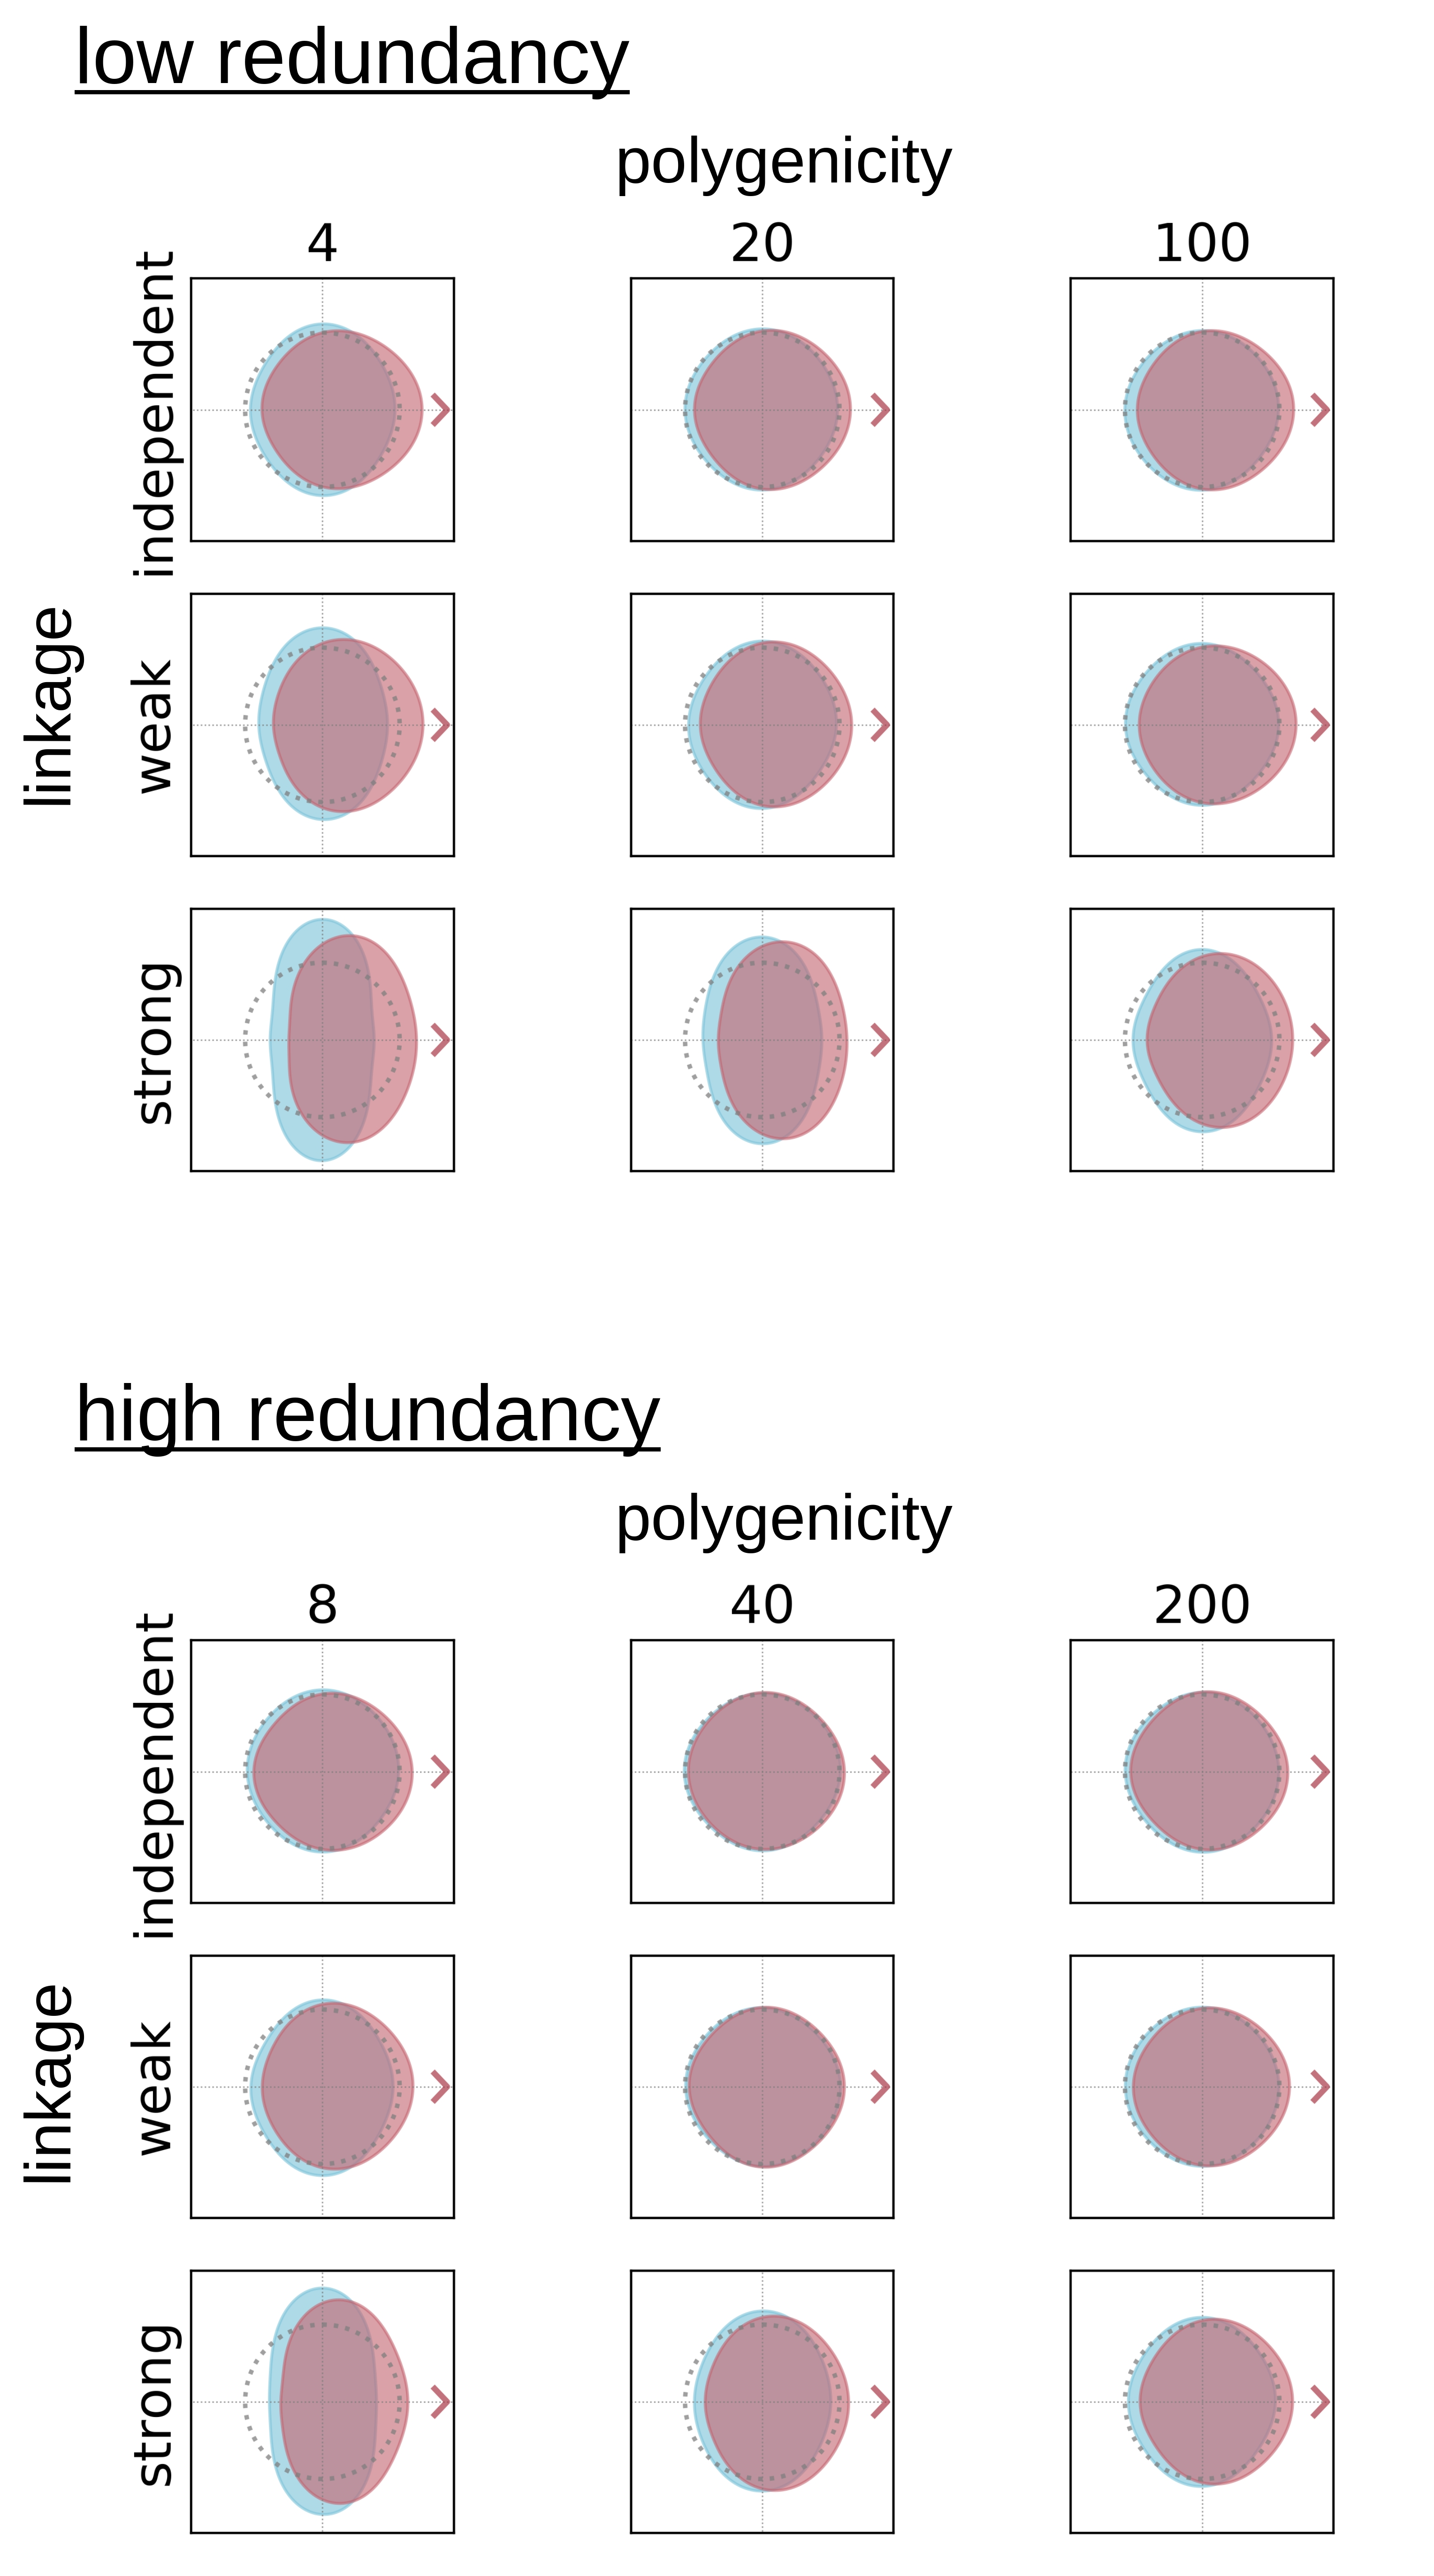
\includegraphics[width=.8\linewidth]{pub/figs_and_stats/FIG_2_gene_flow.jpg}
    \caption{Distributions of gene flow directions during the climate change period of our climate change simulations (red) compared to null simulations (blue) for our 18 scenarios.  The shifting environmental gradient moves to the right (in the direction of the arrow) in our simulations, so rightward gene flow represents up-gradient gene flow, and upward and downward (i.e., `on contour’) gene flow is perpendicular to the environmental gradients. Down-gradient gene flow is expected to be maladaptive under all scenarios, explaining why it is universally suppressed relative to the null results (as evidenced by the blue distributional 'margins' extending to the left of the red distributions in all scenarios). There is a general trend toward increasing on-contour gene flow and decreasing up-gradient gene flow with decreasing linkage and increasing polygenicity.
}
\label{fig:fig_2}
\end{figure}


\subsection*{Linkage and polygenicity}
As expected, our null simulations showed essentially no changes
in mean fitness (Fig. \ref{fig:fig_2}) or population size (Fig. S2), aside from small modeling artefacts that applied to both the 
null and climate-change scenarios, and the phenotypic distributions for the populations in these simulations were
stable through time (Fig. S4).
The results of our climate change simulations exhibited
decreases in population size and mean fitness
that are the expected results of increasing maladaptation \cite{aitken_whitlock}.
They also revealed environment-tracking phenotypic shifts (Fig. \ref{fig:fig_4})
in line with expectations (Fig. \ref{fig:fig_1}),
though these shifts lagged behind environmental change to some extent,
producing suboptimal mean fitness at the end of the climate change period.
Across scenarios, the demographic responses to
climate change increased with increasing linkage
(change in fitness: $\beta_{l} = -0.0018\pm0.0001, P<1\times10^{-15}$;
change in population size: $\beta_{l} = -33.330\pm1.287, P<1\times10^{-15}$).
We also found greater maladaptation, defined as the area in two-dimensional trait space separating the central line
of a population's post-change phenotypic distribution from the central line of the distribution
that would optimally track the changing environment (Figs. \ref{fig:fig_4} and S4), associated with increasing linkage (maladaptation: $\beta_{l} = 0.0038\pm0.0004, P<1\times10^{-15}$).

The magnitude of demographic responses also showed a signal of overall increase with increasing polygenicity
(change in fitness: $\beta_{p} = -0.0022\pm0.0001, P<1\times10^{-15}$;
change in population size: $\beta_{p} = -15.070\pm1.287, P<1\times10^{-15}$;
maladaptation: $\beta_{p} = 0.0097\pm0.0004, P<1\times10^{-15}$),
although the trend was non-monotonic and complex; responses were smallest at moderate polygenicity,
more pronounced at low polygenicity and at high polygenicity when redundancy was high,
and highest at high polygenicity and low redundancy (Figs. \ref{fig:fig_3} and S2).
In fact, under low redundancy and high polygenicity,
populations declined so strongly that adaptive capacity was effectively outstripped,
and the declines persisted throughout
the climate change period, with little indication of evolutionary rescue
(i.e., stabilization and rebound) occurring until the post-change period (Figs. \ref{fig:fig_3} and S2).
The collapse of adaptive capacity in these scenarios
is also visible in the large areas of phenotypic-shift shortfall in Fig. \ref{fig:fig_4}.
The low-redundancy, high-polygenicity, strong-linkage scenario had such low adaptive capacity
that mean fitness declined by 5.2\% on average (from 0.934 to 0.885),
mean population size declined by 17.1\% on average (from 6326 to 5246 individuals),
and the simulated population ceased to occupy the rightmost, fastest-changing portion of the landscape (Fig. \ref{fig:fig_4}).

\begin{figure*}
\centering
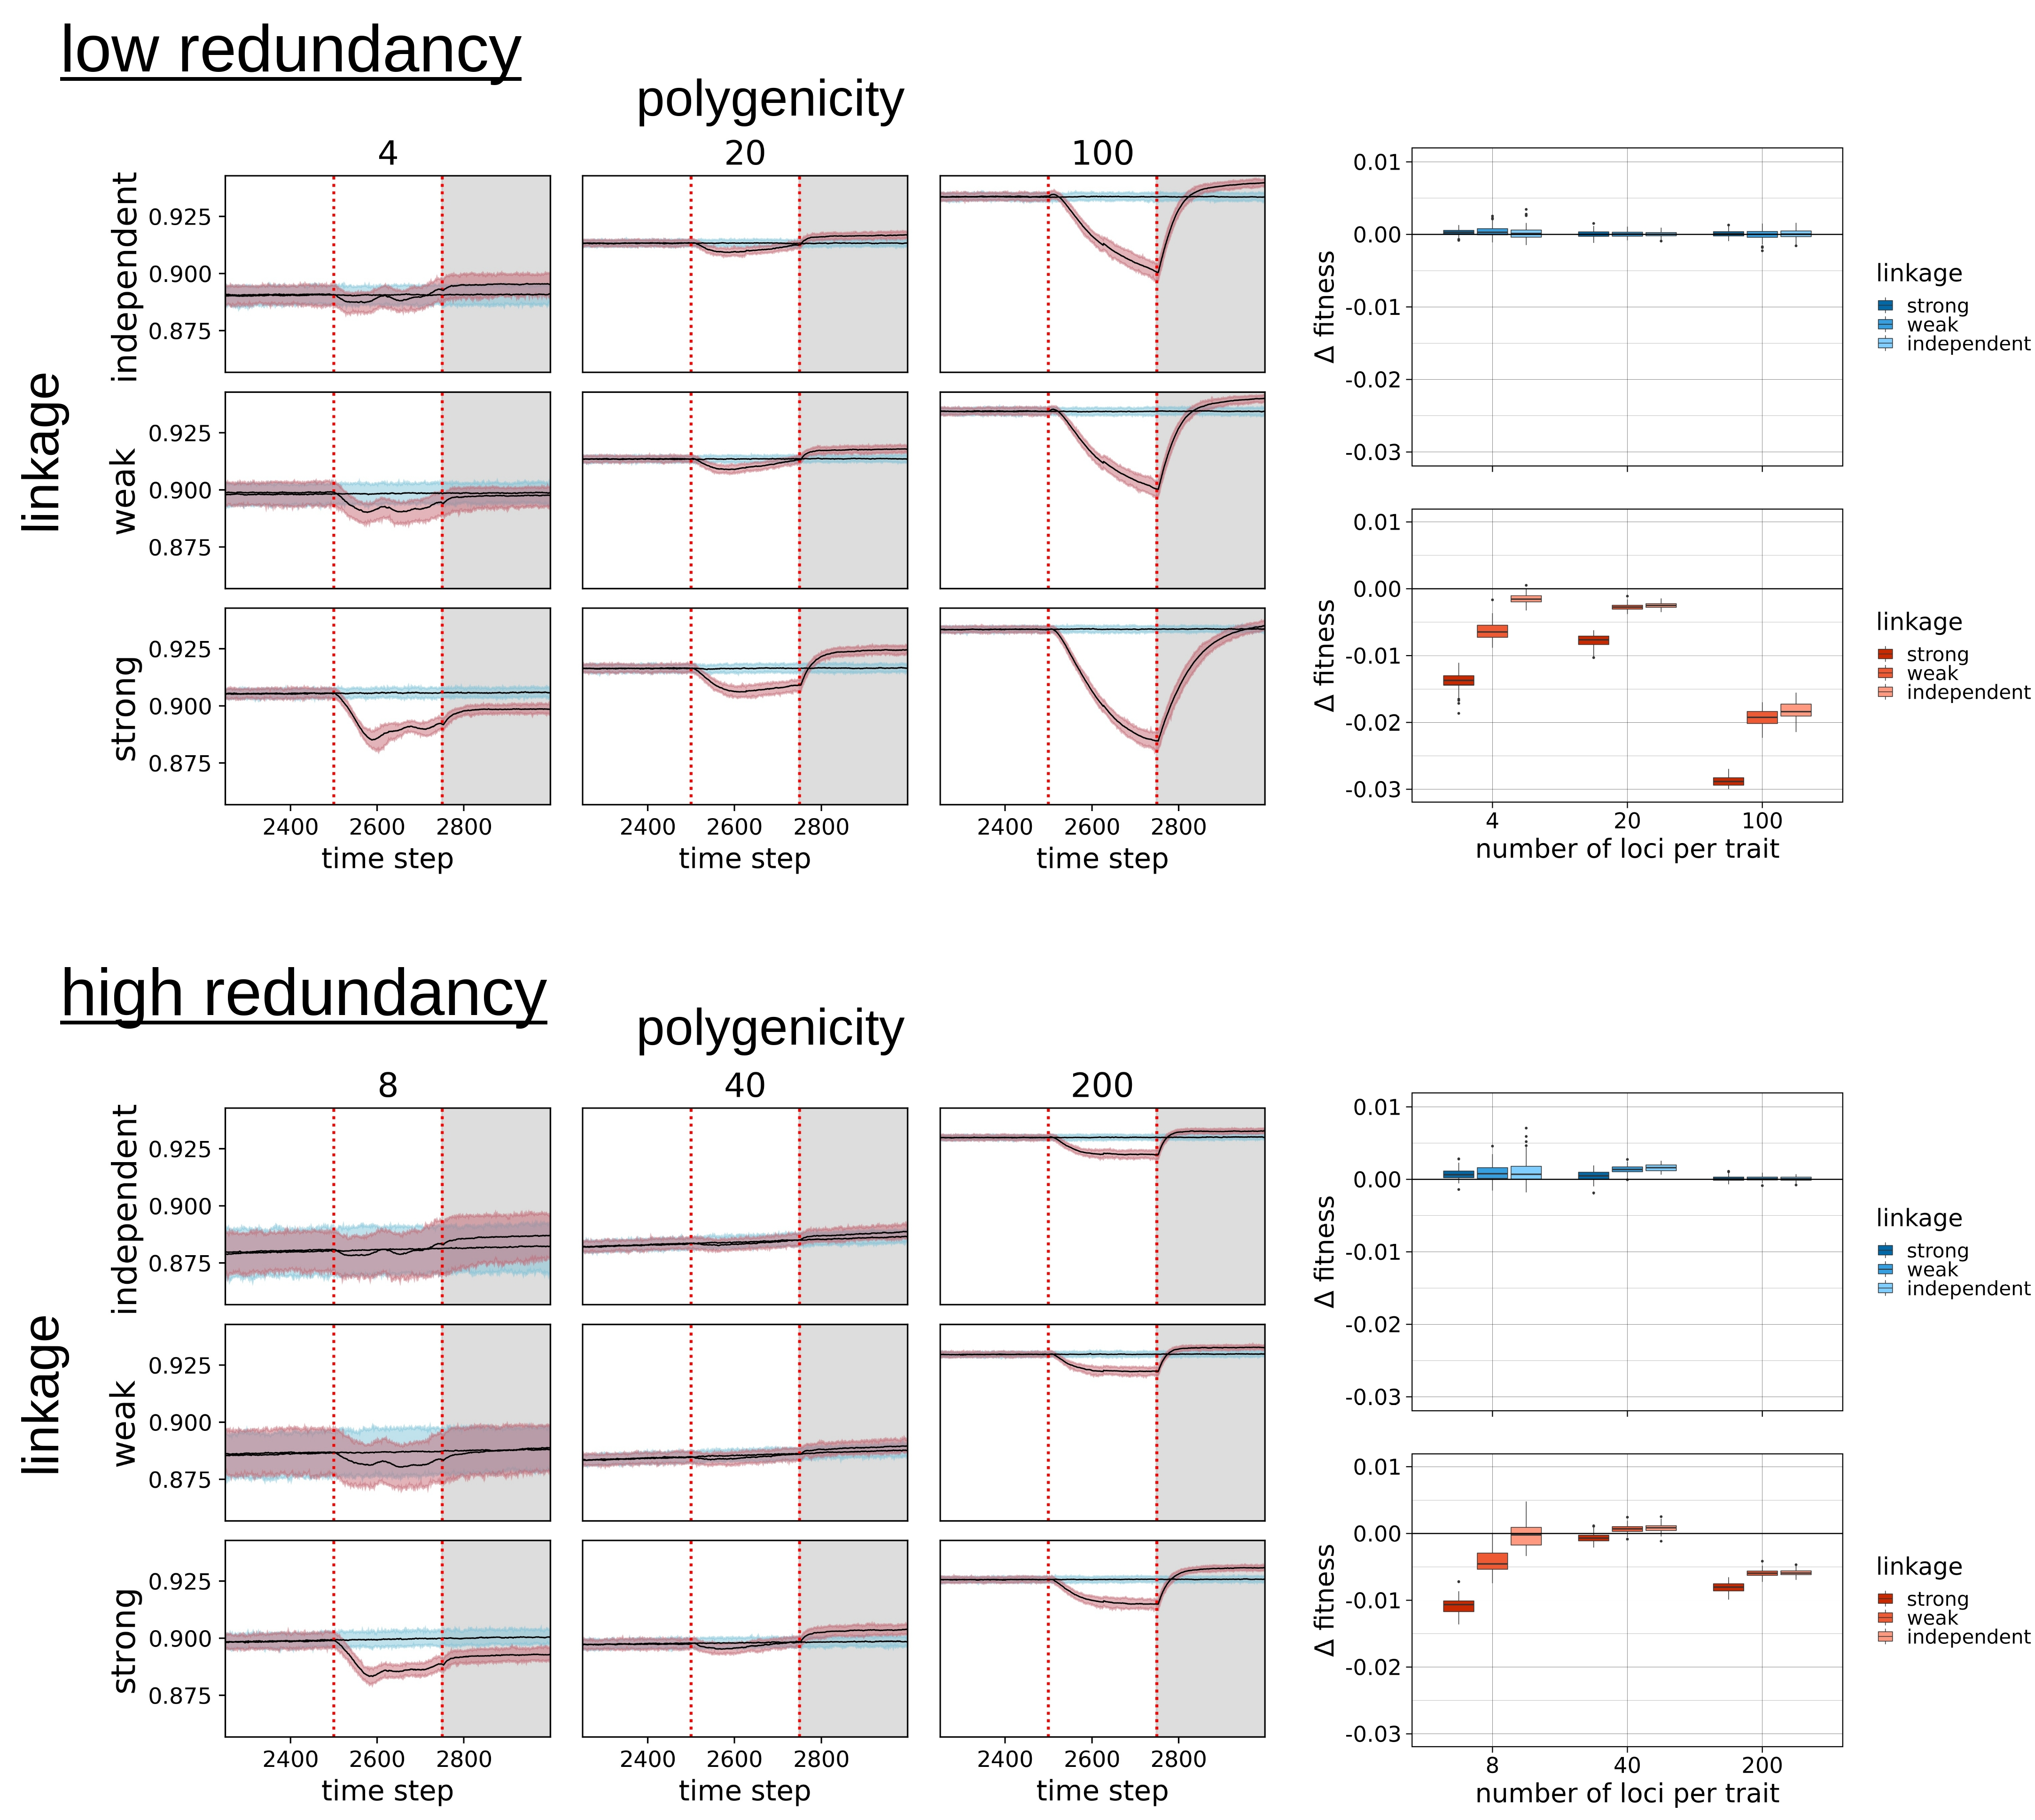
\includegraphics[width=15.8cm]{pub/figs_and_stats/FIG_3_fit_over_time.jpg}
\caption{Left: Mean fitness for all scenarios during the 250 time steps before, during, and after the climate change period (separated by red, dashed lines). Black lines represent the mean values, and the shaded red and blue areas represent variability envelopes (5th percentile to
95th percentile) for all replicates for climate change and null simulations, respectively.  Right: Boxplots of changes in mean fitness during the climate change period for all scenarios. Null scenarios are plotted on the top in blue, and main scenarios are plotted on the bottom, in red. Within each plot, the scenarios are organized by polygenicity (number of loci per trait) on the x-axis and shaded by the strength of linkage.
}
\label{fig:fig_3}
\end{figure*}

\begin{figure*}
\centering
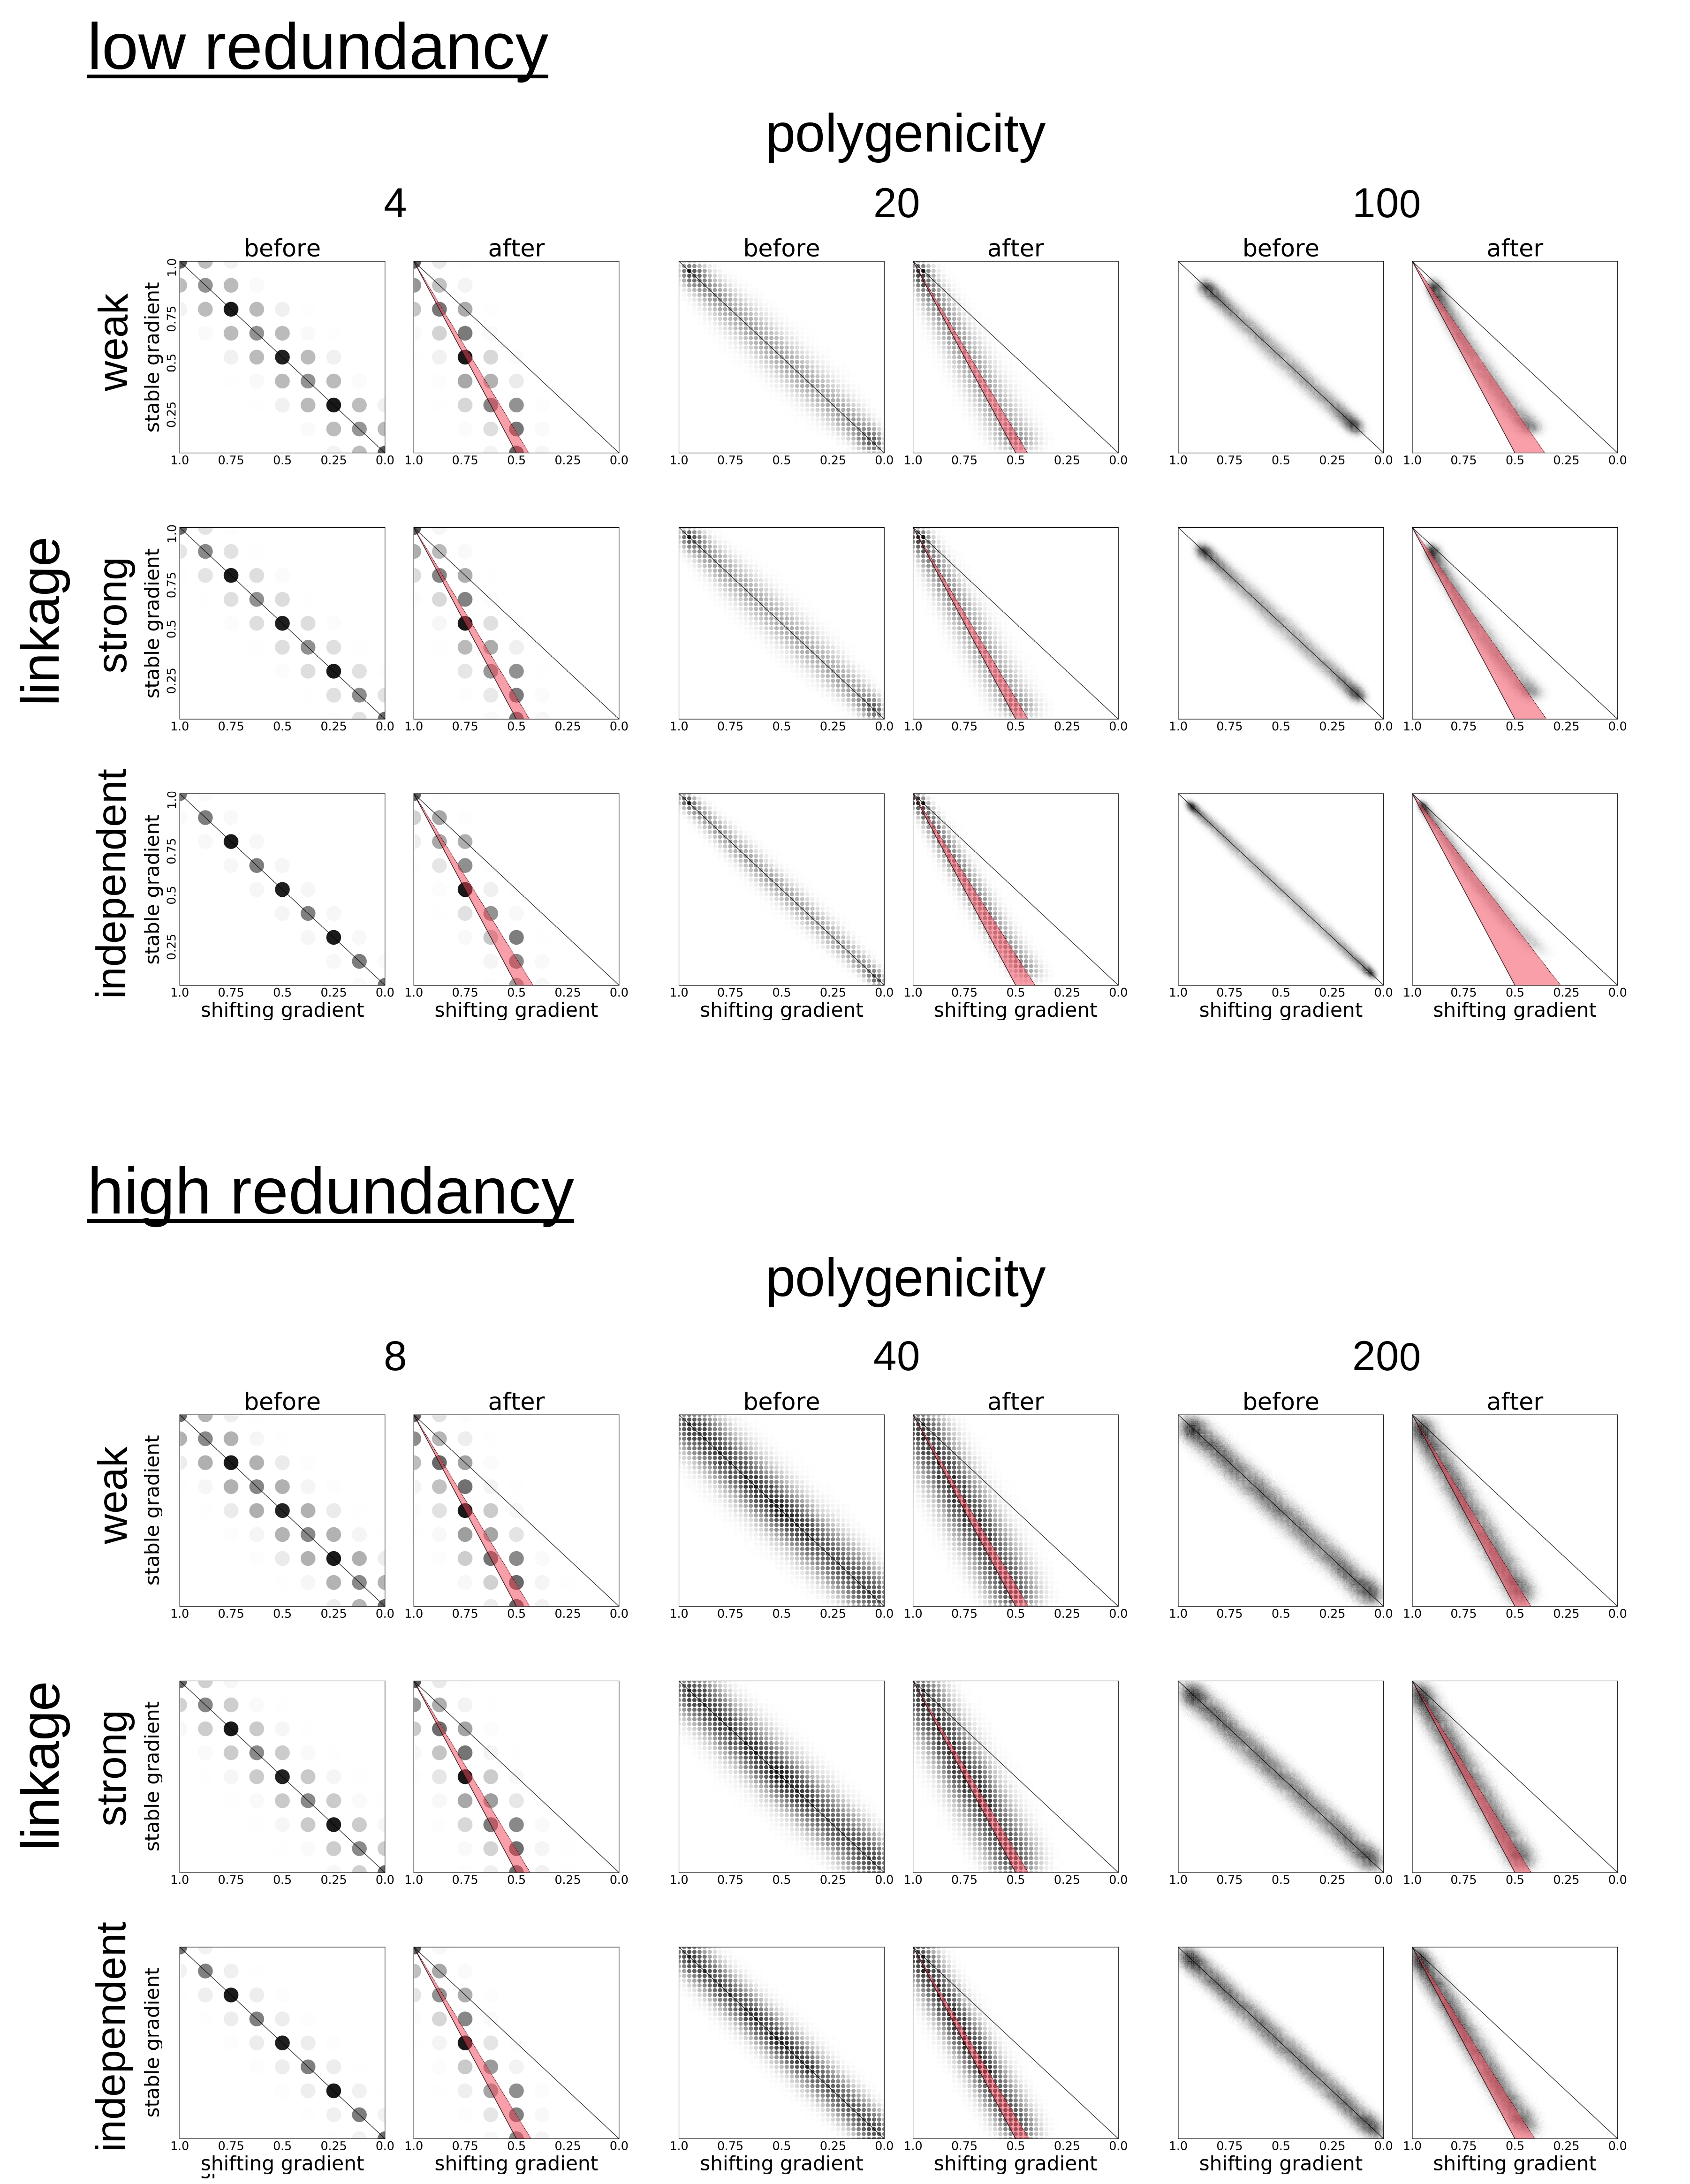
\includegraphics[width=15.8cm]{pub/figs_and_stats/FIG_4_phenotypic_shift.jpg}
\caption{Scatterplots of the observed versus expected phenotypic shift during the climate change period for all 18 of our simulated scenarios. For each scenario, the left ('before') scatterplot shows the distribution of phenotypes before climate change begins, and the right ('after') scatterplot shows how the distribution has shifted by the end of the climate change period. The trait adapted to the shifting environmental gradient is distributed along the x-axis, with the trait adapted to the stable gradient on the y-axis. Each plot is an ensemble of the results for all 100 replicates of each scenario. The size and opacity of each point represents the number of individuals exhibiting that two-dimensional phenotype. The gridded arrangement of the points in each scatterplot is a function of the number of loci per trait, which determines the set of possible phenotypes. Solid black lines delineate the shifts in the phenotypic distributions’ central tendencies that are expected to take place during the climate change period, dotted black lines depict the observed distributions’ central tendencies, and red wedges depict the differences between the expected and observed distributions (‘phenotypic shortfall’).
}
\label{fig:fig_4}
\end{figure*}

\subsection*{Genotypic redundancy}
Our high-redundancy scenarios showed
consistently smaller demographic responses to climate change, and higher adaptive capacity,
than their low-redundancy counterparts 
(change in fitness: $\beta_{r} = 0.0040\pm0.0002, P<1\times10^{-15}$;
change in population size: $\beta_{r} = 39.060\pm2.101, P<1\times10^{-15}$;
maladaptation: $\beta_{r} = -0.0098\pm0.0006, P<1\times10^{-15}$), consistent with our hypothesis that
genotypic redundancy can facilitate adaptation to shifting environmental gradients (Figs. \ref{fig:fig_2} and S2).
This effect was most pronounced in the high-polygenicity scenarios,
which exhibited much milder demographic decline under high redundancy compared to low redundancy,
despite still showing no evidence of demographic rebound until after climate change (Fig. \ref{fig:fig_3}).
Indeed, increased redundancy put the demographic
impacts of these scenarios on par with those
of the low polygenicity scenarios (Figs. \ref{fig:fig_3} and S2).


\section*{Discussion}

Current theoretical understanding of evolutionary responses to climate change
largely derives from a simplified mechanistic model in which
adaptation is universally facilitated by up-gradient gene flow.
This model also serves as the inspiration for some climate-smart
approaches to biodiversity management
(e.g., assisted gene flow; \cite{aitken_whitlock}).
However, adopting this model as the basis
for theoretical and mechanistic research
risks overlooking the influence of
genomic architecture on multivariate adaptation to environmental change.
Starting from a more realistic, multi-trait framework,
our simulations demonstrate that up-gradient gene flow does indeed
occur under climate change
but that its contributions to local adaptation and persistence may be constrained
by polygenicity and, to a lesser extent, linkage.
Given the plausible range of genomic architectures we simulate
\cite{barghi_polygenic,boyle,rockman,savolainen,sella,bomblies},
these results raise the compelling
possibility that up-gradient gene flow, while unlikely
to be entirely maladaptive, could play a limited role in
climate change adaptation in many systems.
This may be especially true in systems where climate-adapted traits
have more dispersed architectures --- for example, architectures composed of many genes of small effect \cite{yeaman_review}.
This poses an important question for subsequent research:
how often are the genomic architectures underlying climate-adapted traits dispersed
versus concentrated?

We also show that the genomic architecture of climate-adapted traits
can influence the nature and size of demographic responses
to climate change.
Our results suggest that strong linkage between non-neutral loci,
especially under high polygenicity, can increase maladaptation and demographic decline
during climate change. 
In the most extreme case, evolutionary rescue was absent;
high polygenicity and low redundancy
combined to drive dramatic and persistent demographic declines,
and even caused local extinction when linkage was strong.
This was unexpected in light of previous work reporting
that dispersed architectures produce stable,
resilient phenotypic clines despite transient genotypic composition \cite{yeaman_amnat,yeaman_review}
and, thus, that species with such architectures
could exhibit rapid local adaptation \cite{aitken_yeaman}.
We did nonetheless expect evolutionary responses to climate change
to be slower in these scenarios,
because natural selection is less effective on smaller-effect alleles,
gene flow may be more swamping for these alleles,
and high linkage leads to longer expected wait times for the generation
of novel, adaptive recombinant genotypes.
But we did not expect
adaptive capacity to be completely outstripped.
However, it appears that the rate of environmental change simply exceeded the pace of
adaptation. This is evidenced by the the quick demographic rebound
that occurred in the  
`post-change' periods (Fig. 3), a rebound was likely driven by the same evolutionary dynamics
that occur during evolutionary rescue, but that in these extreme scenarios
probably only emerged once environmental change had ceased.

Remarkably, we also observed higher maladaptation and larger demographic declines
in our low-polygenicity scenarios with fewer, larger-effect alleles.
Demographic decline was least pronounced
in our moderate-polygenicity models.
This contrasts with previous work finding that adaptation
to a gradient is more effective under either
concentrated or dispersed genomic architectures \cite{yeaman_whitlock}.
This disagreement may be attributable to the
difference in timeframes between adaptation to a univariate environmental gradient
and adaptation to a decoupled, multivariate gradient.
Adaptation to a single, static gradient can proceed gradually,
so may either favor large-effect alleles or allele-clusters in the long haul,
once they have arisen by mutation, recombination, gene flow, or a combination thereof \cite{yeaman_amnat,yeaman_review},
or dispersed architectures in temporally fluctuating environments \cite{burger,kondrashov,yeaman_review,yeaman_whitlock}.
However, the sudden onset of persistent environmental change 
in a population that is already locally adapted triggers a 'race against time,' 
and genomic architectures with
optimal adaptive capacity may be the 'middle ground' architectures that comprise
freely recombining loci with small enough effect sizes to avoid large declines in fitness from migration load
but with large enough effect sizes to allow for effective natural selection and to avoid the long wait times necessary
for recombination to cluster many adaptive loci into larger-effect haplotypes.
This presents the surprising possibility that an 'evolutionary trade-off' may exist, such
that mid-effect-size alleles may confer maximal adaptive capacity to environmental
change, and suggests interesting avenues for future work.

The fact that high genomic redundancy reduces demographic decline,
across all scenarios, contributes to the growing recognition of the importance of redundancy
as a driver of evolutionary outcomes for polygenic traits
\cite{laruson,yeaman_review}.
This also presents a possible mechanism to be explored
in real-world populations living at colder range edges.
Much like the local populations in the rightmost region of our low-redundancy scenarios,
these local populations could already be at the edge of the phenotypic space defined by
their standing genetic variation;
in this case, 
segregating redundancy (\cite{laruson}) and, thus,
adaptive capacity would be low,
so vulnerability to local extinction would be substantial.
However, species whose cold range edges are predominantly determined by geographic barriers
or biotic interactions rather than by climate limits \cite{thomas}
could feature local populations more similar to our high-redundancy scenarios;
segregating redundancy would be higher,
so selection would be balancing rather than directional, and adaptive capacity would be substantial.
This logic implies that textit{in situ} adaptation would be a substantial contributor to
adaptive capacity in these scenarios --- an implication supported by the fact that
we observed reduced up-gradient gene flow across all high-redundancy scenarios.

Our findings also help advance the theoretical understanding
of local adaptation with recombination.
Recombination is generally regarded as disadvantageous
in situations of clinal adaptation
with gene flow, because it disrupts the
association between adaptive loci 
underlying a single trait \cite{tigano}.
Unstable environments experiencing stochastic temporal fluctuations
are considered a major exception \cite{tigano},
but our results suggest that this may also extend
to environments undergoing monotonic change
such as that caused by climate change.
In fact, recombination may
be advantageous under these conditions,
particularly when species have distinct traits simultaneously adapted
to distinct and decoupling gradients.
This advantage likely arises because recombination
allows for more effective \textit{in situ} adaptation
by shifting allelic covariance, despite the fact that
it still disrupts the associations between loci
that would otherwise allow for the development of
larger-effect gene clusters.
This suggests that \textit{in situ} shifts in allelic covariance
provide an alternative to adaptive gene flow as a mechanism for evolutionary rescue,
especially in multi-trait systems where gene flow can be adaptive
for shifting climatic gradients but maladaptive with
respect to other, decoupled gradients.

A major challenge in simulation-based research is the complexity of the high-dimensional 
parameter space that could be explored.
Useful and informative studies can be constructed by focusing on a small set of
key parameters while holding others at reasonable values, as we have done here.
This nonetheless leaves unexplored a number of secondary parameters
that can have non-negligible influence over the complex ecological phenomena of interest.
In the case of evolutionary responses to climate change
this provides various areas for future research
These include
population size, which is a key determinant of the relative strengths of drift
and natural selection \cite{murray} and of the wait time to emergence of
recombinant haploytpes \cite{christiansen};
movement behavior, a key factor influencing
migration-selection dynamics \cite{wright,haldane,barton};
allelic effect size distributions \cite{orr},
which are omitted here in favor of a single, fixed effect size;
and the spatiotemporal structure of the environment,
including gradients' geometries, slopes, orientations, and rates of change
(e.g., \cite{benes}).
Additionally, important and conservation-relevant insight could emerge from the 
integration of other dimensions of climate change ecology, including range shifts 
\cite{weiss-lehman}, plasticity \cite{chevin},
and range-wide variation in population density \cite{aitken_whitlock}.
Finally, more complex evolutionary scenarios could also be explored, including 
pleiotropy \cite{thompson} and epistasis,
hybridization \cite{turbek}, life history variation,
and even scenarios in which the multiple traits differ in the
complexity of their genomic architectures --- a realistic
arrangement that could exhibit different
evolutionary outcomes than the ones we describe here.

\section*{Conclusions}
Gene flow and adaptation are two of the main mechanisms by which species may persist under climate change. Evaluating the conditions under which they are likely to contribute to species persistence is essential for better understanding 
microevolutionary responses to climate change and for informing management. Our simulations show that 
genomic architecture can play an important, but largely overlooked, role in influencing evolutionary outcomes.
This includes determining the relative effectiveness
of up-gradient gene flow and \textit{in situ} adaptation,
the magnitude and persistence
of maladaptation,
and the likelihood of concomitant demographic decline
or evolutionary rescue.
These findings highlight the importance of considering multivariate environmental gradients
for climate change research, and suggest that the genomic architecture underlying traits
adapted to those gradients has direct consequences for how species respond to environmental change.
Broader crosstalk between the literature on climate change ecology
and the literature on adaptive genetic architectures can help
construct a sounder and more comprehensive understanding of
whether, where, and how species may adapt to climate change.


\acknow{We thank A. P. Bishop, T. Dawson,  J. Frederick, N. Graham, M. Kelly, M. McElroy, E. Westeen, G. Wogan, and M. Yuan for feedback and guidance on various iterations of the simulations presented herein. We thank Berkeley Research Computing for providing access to the Savio computing cluster. We thank D. Ehrenfeld, N. Fefferman, M. Fitzpatrick, and L. Plough for cultivating an interest in conservation genetics. Lastly, we thank M. Terasaki Hart, C. Nemec-Hart, G. Hart, J. Hart, and M. Tylka for supporting and encouraging a lifetime of curiosity about nature, and C. S. aTunde Adjuah, B. Evans, R. Pérez Joglar, Y. Y. Ma, and J. Redman for the great company during long periods of solitude. This work was supported by a Berkeley Fellowship from University of California, Berkeley (to D.E.T.H.) and by National Science Foundation grant DEB1845682 (to I.J.W.).}

\showacknow{} % Display the acknowledgments section

% Bibliography
\bibliography{terasaki_hart_genarch_climchng}

\end{document}
